\begin{frame}{Using nhls: Setup}
  \begin{columns}
  \column{0.38\linewidth}
  \begin{outline}
  \1 Generic over grid dimension 
  \1 Generic over stencil
  \1 Need stencil at compile time
  \2 For now...
  \1 Solvers are made for a fixed number of steps
  \end{outline}

  \column{0.58\linewidth}
  \begin{center}
  \centering
  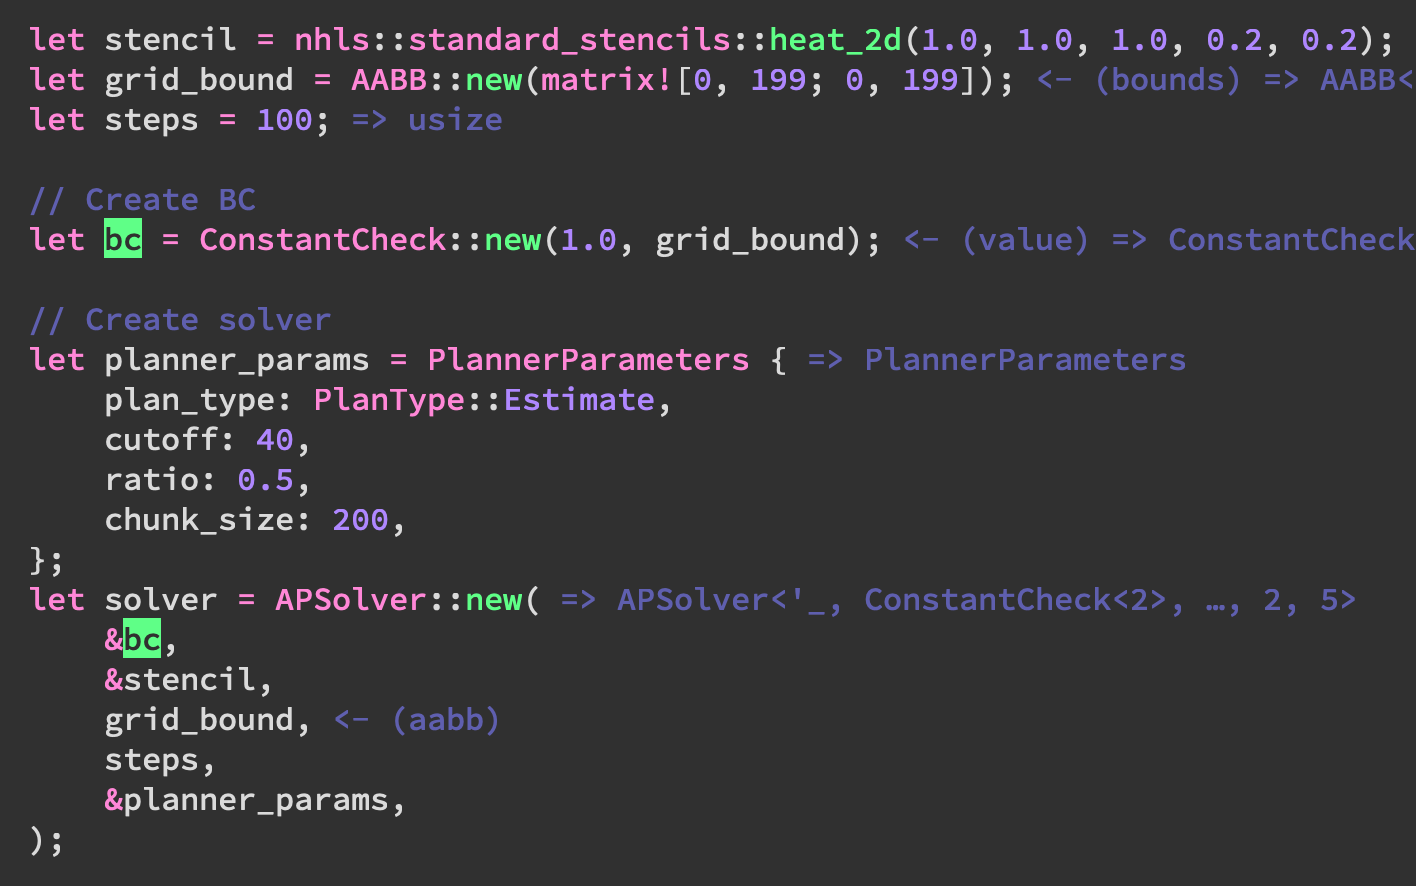
\includegraphics[width=\textwidth]{nhls_setup.png}
  \end{center}
\end{columns}
\end{frame}

\begin{frame}{Using nhls: Apply Solver}
  \begin{columns}
  \column{0.38\linewidth}
  \begin{outline}
  \1 Solvers can be applied many times 
  \1 No additional allocations 
  \end{outline}

  \column{0.58\linewidth}
  \begin{center}
  \centering
  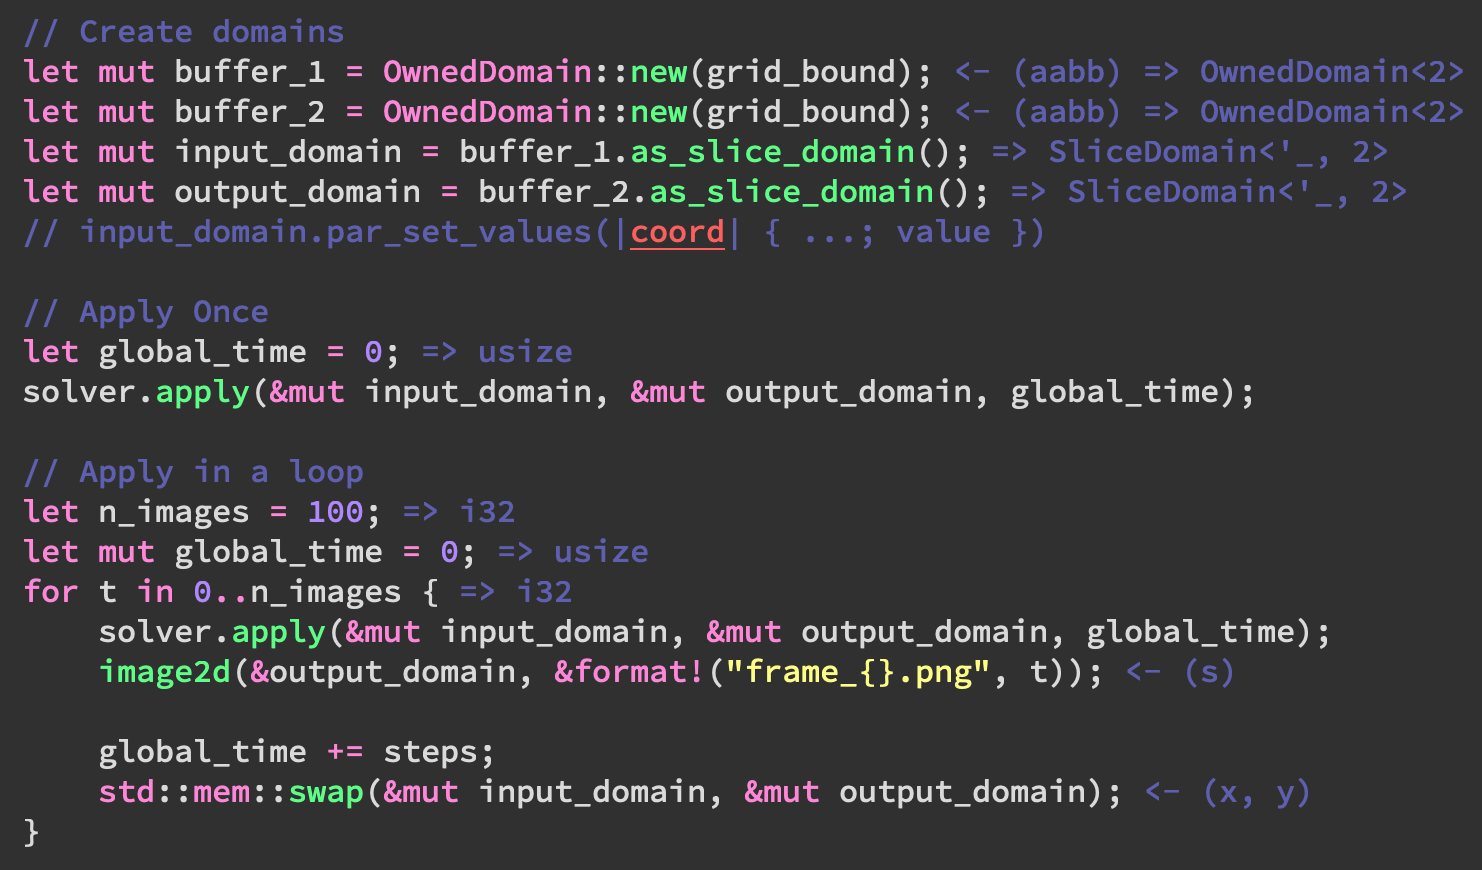
\includegraphics[width=\textwidth]{nhls_solver.png}
  \end{center}
\end{columns}
\end{frame}

\placelogofalse
\begin{frame}{Using nhls: Time varying BC}
  \begin{columns}
  \column{0.48\linewidth}
  \begin{center}
  \centering
  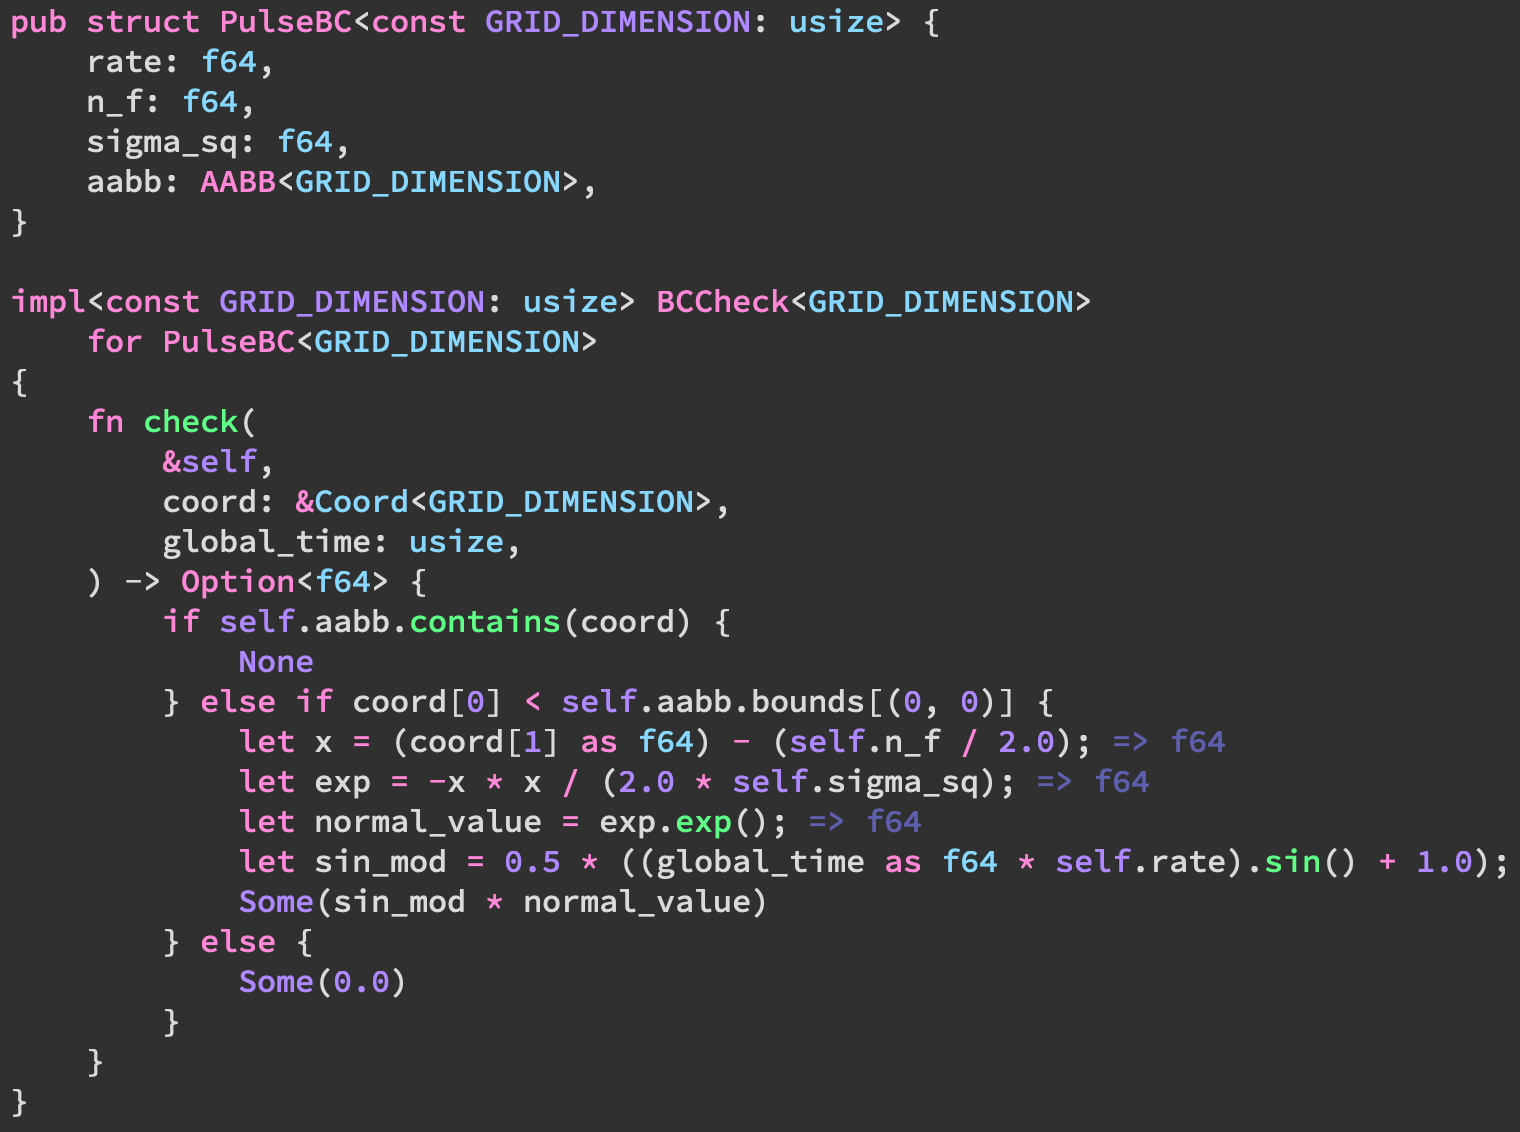
\includegraphics[width=\textwidth]{nhls_time_vary_bc.png}

  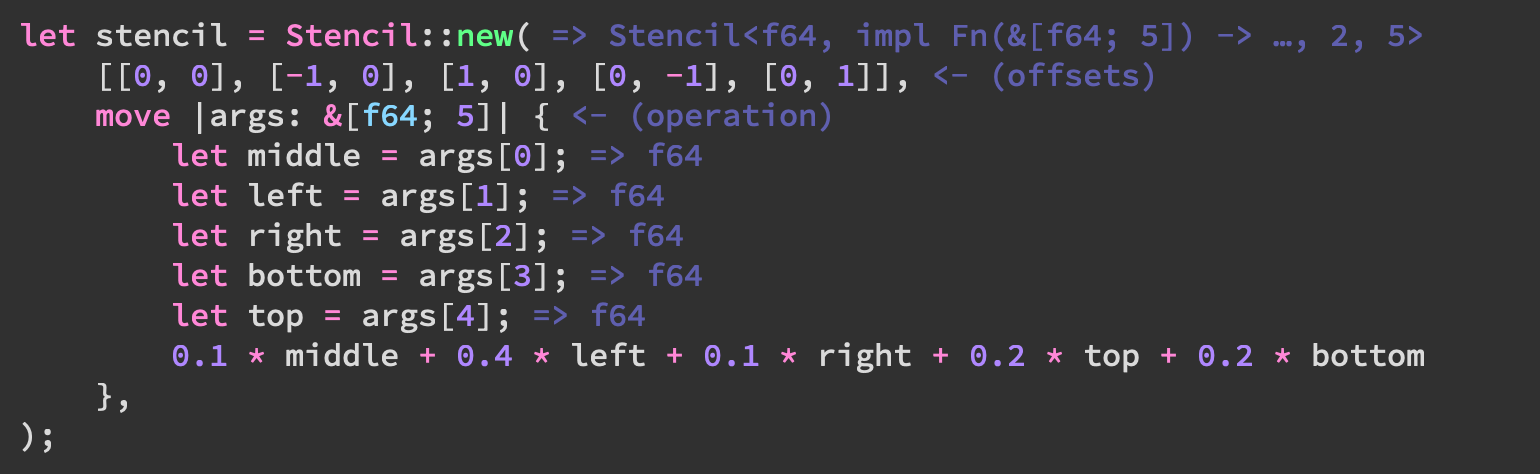
\includegraphics[width=\textwidth]{nhls_shift_stencil.png}
  \end{center}

  \column{0.48\linewidth}
  \begin{center}
  \centering
  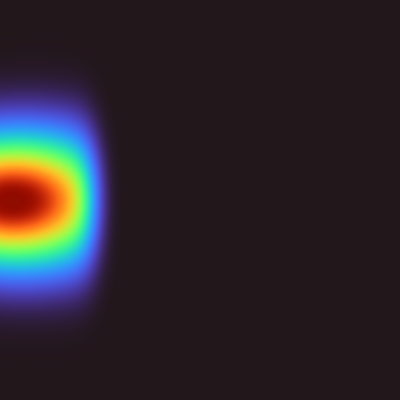
\includegraphics[width=0.5\textwidth]{frame_0006.png}

  $t = 250$

  \vspace{0.5cm}

  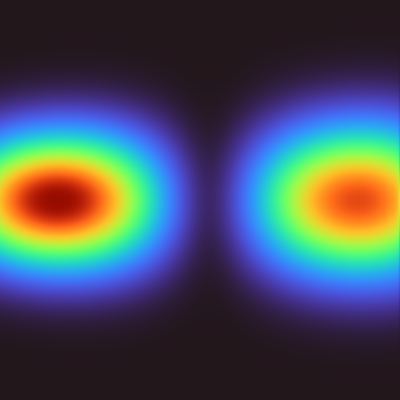
\includegraphics[width=0.5\textwidth]{frame_0029.png}

  $t = 1400$ 
  \end{center}
\end{columns}
\end{frame}
\placelogotrue
